%-------------------------
% Resume in Latex
% Author
% License : MIT
%------------------------

%---- Required Packages and Functions ----

\documentclass[a4paper,11pt]{article}
\usepackage{latexsym}
\usepackage{xcolor}
\usepackage{float}
\usepackage{ragged2e}
\usepackage[empty]{fullpage}
\usepackage{wrapfig}
\usepackage{lipsum}
\usepackage{tabularx}
\usepackage{titlesec}
\usepackage{geometry}
\usepackage{marvosym}
\usepackage{verbatim}
\usepackage{enumitem}
%\usepackage[hidelinks]{hyperref}
\usepackage{hyperref}
\usepackage{fancyhdr}
\usepackage{fontawesome5}
\usepackage{multicol}
\usepackage{graphicx}
\usepackage{cfr-lm}
\usepackage[T1]{fontenc}
\usepackage{pdfpages}
\usepackage[style=authoryear,sorting=ynt, maxbibnames=5]{biblatex}
\setlength{\multicolsep}{0pt} 
\pagestyle{fancy}
\fancyhf{} % clear all header and footer fields
\fancyfoot{}
\renewcommand{\headrulewidth}{0pt}
\renewcommand{\footrulewidth}{0pt}
\geometry{left=1.4cm, top=0.8cm, right=1.2cm, bottom=1cm}
% Adjust margins
%\addtolength{\oddsidemargin}{-0.5in}
%\addtolength{\evensidemargin}{-0.5in}
%\addtolength{\textwidth}{1in}
\usepackage[most]{tcolorbox}
\tcbset{
	frame code={}
	center title,
	left=0pt,
	right=0pt,
	top=0pt,
	bottom=0pt,
	colback=gray!20,
	colframe=white,
	width=\dimexpr\textwidth\relax,
	enlarge left by=-2mm,
	boxsep=4pt,
	arc=0pt,outer arc=0pt,
}

\definecolor{linkcolour}{rgb}{0,0.2,0.6}
\hypersetup{colorlinks,breaklinks,urlcolor=linkcolour,linkcolor=linkcolour}
\usepackage[style=authoryear,sorting=ynt, maxbibnames=5]{biblatex}
\urlstyle{same}

\raggedright
\setlength{\tabcolsep}{0in}


% Sections formatting
\titleformat{\section}{
  \vspace{-4pt}\scshape\raggedright\large
}{}{0em}{}[\color{black}\titlerule \vspace{-7pt}]

%-------------------------
% Custom commands
\newcommand{\resumeItem}[2]{
  \item{
    \textbf{#1}{\hspace{0.5mm}#2 \vspace{-0.5mm}}
  }
}

\newcommand{\resumePOR}[3]{
\vspace{0.5mm}\item
    \begin{tabular*}{0.97\textwidth}[t]{l@{\extracolsep{\fill}}r}
        \textbf{#1}\hspace{0.3mm}#2 & \small{#3}
    \end{tabular*}
    \vspace{-2mm}
}


% \newcommand{\resumePOR}[3]{
% \vspace{0.5mm}\item
%     \begin{tabular*}{0.97\textwidth}[t]{l@{\extracolsep{\fill}}r}
%         \textbf{#1}\hspace{0.3mm}#2 & \textit{\small{#3}} 
%     \end{tabular*}
%     \vspace{-2mm}
% }

\newcommand{\resumeSubheading}[4]{
\vspace{0.5mm}\item
    \begin{tabular*}{0.98\textwidth}[t]{l@{\extracolsep{\fill}}r}
        \textbf{#1} & \footnotesize{#4} \\
        \textit{\footnotesize{#3}} &  \footnotesize{#2}\\
    \end{tabular*}
    \vspace{-2.4mm}
}

% \newcommand{\resumeSubheading}[4]{
% \vspace{0.5mm}\item
%     \begin{tabular*}{0.98\textwidth}[t]{l@{\extracolsep{\fill}}r}
%         \textbf{#1} & \textit{\footnotesize{#4}} \\
%         \textit{\footnotesize{#3}} &  \footnotesize{#2}\\
%     \end{tabular*}
%     \vspace{-2.4mm}
% }

\newcommand{\resumeProject}[4]{
\vspace{0.5mm}\item
    \begin{tabular*}{0.98\textwidth}[t]{l@{\extracolsep{\fill}}r}
        \textbf{#1} & \footnotesize{#3} \\
        \emph{\footnotesize{#2}} & \footnotesize{#4}
    \end{tabular*}
    \vspace{-2.4mm}
}

% \newcommand{\resumeProject}[4]{
% \vspace{0.5mm}\item
%     \begin{tabular*}{0.98\textwidth}[t]{l@{\extracolsep{\fill}}r}
%         \textbf{#1} & \textit{\footnotesize{#3}} \\
%         \footnotesize{\textit{#2}} & \footnotesize{#4}
%     \end{tabular*}
%     \vspace{-2.4mm}
% }


\newcommand{\resumeGit}[4]{
\vspace{0.5mm}
    \begin{tabular*}{0.98\textwidth}[t]{l@{\extracolsep{\fill}}r}
        \footnotesize{#1} & \footnotesize{#2} \\
        \footnotesize{#3} & \footnotesize{#4}
    \end{tabular*}
    \vspace{-2.4mm}
}

\newcommand{\resumeSubItem}[2]{\resumeItem{#1}{#2}\vspace{-4pt}}

% \renewcommand{\labelitemii}{$\circ$}
\renewcommand{\labelitemi}{$\vcenter{\hbox{\tiny$\bullet$}}$}

\newcommand{\resumeSubHeadingListStart}{\begin{itemize}[leftmargin=*,labelsep=0mm]}
\newcommand{\resumeHeadingSkillStart}{\begin{itemize}[leftmargin=*,itemsep=1.7mm, rightmargin=2ex]}
\newcommand{\resumeItemListStart}{\begin{justify}\begin{itemize}[leftmargin=3ex, rightmargin=2ex, noitemsep,labelsep=1.2mm,itemsep=0mm]\small}
\newcommand{\resumePara}{\begin{justify}\small}

\newcommand{\resumeSubHeadingListEnd}{\end{itemize}\vspace{2mm}}
\newcommand{\resumeHeadingSkillEnd}{\end{itemize}\vspace{-2mm}}
\newcommand{\resumeItemListEnd}{\end{itemize}\end{justify}\vspace{-2mm}}
\newcommand{\resumeParaEnd}{\end{justify}}
\newcommand{\cvsection}[1]{%
\vspace{2mm}
\begin{tcolorbox}
    \textbf{\large #1}
\end{tcolorbox}
    \vspace{-4mm}
}

\newcolumntype{L}{>{\raggedright\arraybackslash}X}%
\newcolumntype{R}{>{\raggedleft\arraybackslash}X}%
\newcolumntype{C}{>{\centering\arraybackslash}X}%
%---- End of Packages and Functions ------

%-------------------------------------------
%%%%%%  CV STARTS HERE  %%%%%%%%%%%
%%%%%% DEFINE ELEMENTS HERE %%%%%%%
\newcommand{\name}{Robert McGregor} % Your Name
\newcommand{\course}{A/Principal Remote Sensing Officer} % Your Program
\newcommand{\roll}{Initiating land clearing detection} % Your Roll No.
\newcommand{\phone}{0467264511} % Your Phone Number
\newcommand{\emailb}{robert.mcgregor@outlook.com.au} %Email 1
\newcommand{\emaila}{robert.mcgregor@nt.gov.au} %Email 2

% \usepackage{natbib}
% \bibliographystyle{agsm}
% \title{Bibliography management: \texttt{natbib} package}

%for publications


\begin{document}
%\fontfamily{lmss}\selectfont
%\fontfamily{crm}\selectfont
%----------HEADING-----------------


\parbox{2.35cm}{%
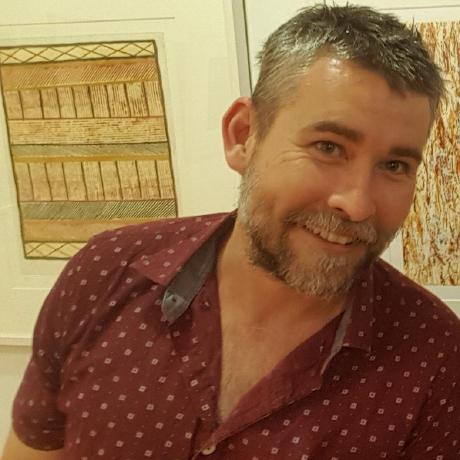
\includegraphics[width=2cm,clip]{profile_picture.jpg}
}
\parbox{\dimexpr\linewidth-2.8cm\relax}{
\begin{tabularx}{\linewidth}{L r} \\
  \textbf{\Large \name} & {\href{tel:0467264511}{\raisebox{-0.05\height}\faMobile \ 0467264511}} \\%\raisebox{0.0\height}{\footnotesize \faPhone}\ +61-\phone} \\
  {} & \href{mailto:\emaila}{\raisebox{0.0\height}{\footnotesize \faEnvelope}\ {\emaila}} \\
  \course &  \href{mailto:\emailb}{\raisebox{0.0\height}{\footnotesize \faEnvelope}\ {\emailb}}\\
  {Rangelands Division,} &  \href{https://yourGithubProfile.com/}{\raisebox{0.0\height}{\footnotesize \faGithub}\ {robotmcgregor}} \\
  {Department of Environment Parks and Water Security, Northern Territory Government} & \href{https://www.linkedin.com/in/robotmcgregor/}{\raisebox{0.0\height}{\footnotesize \faLinkedin}\ {robotmcgregor}}
\end{tabularx}
}
% \parbox{3.0cm}{%
% \flushright \includegraphics[width=2cm,clip]{nitp_logo.png}
% }



%----------- selection criteria ----------------
\section{\textbf{Selection Criteria}}
\subsection{Knowledge and experience}
\begin{enumerate}

\item  I have extensive experience in the production of remotely sensed products using Python and multiple
GIS software packages (ArcMap, ArcMap Pro and QGIS). For example, I regularly write and run
Python scripts and pipelines to produce seasonal composites, resample satellite imagery and produce multiple remotely sensed products for multiple monitoring projects for the Northern Territory Government (NTG).

\item I have significant experience in writing and running Python pipelines to extract zonal statistics from remotely sensed products. I also have extensive experience in applying vegetation indices and performing time trace analysis for monitoring land condition and land clearing events.

\item I have significant experience in remotely sensed product validation when analysing machine learning models, for example validating regression predictions with Root Mean Square Error (RSME), coefficient of determination $(R^{2})$, Mean Absolute Error (MAE) and Mean Squared Error (MSE). Alternatively using accuracy, recall, precision, F1 score and the Matthews correlation coefficient metrics for classification predictions. Further to this, I also have experience with field validation of data products.

\item I have a well developed understanding and experience in the development life cycle of remotely sensed data products, from pre-processing, analysis, documentation, production of metadata and publishing. I am currently responsible for managing DEPWS's Raster directory which contains approximately 50 TB of remotely sensed data products. Each raster undergoes some level of Python based processing either on the Queensland (QLD) Remote Sensing Centre (RSC) High Performance Computer (HPC) - Athena52 or on one of the three NTG Remote Sensing Unit (RSU) virtual machines, which I am also responsible for. All of our data production is accomplished using Python scripts, pipelines and notebooks, and includes, data collation or production, masking, re-sampling, compositing, adding metadata, updating documentation (Confluence/Knowledge WIKI) and publishing. 

\end{enumerate}
\subsection{Skills and capabilities}
\begin{enumerate}

\item I have extensive experience across the suite of remote sensing and GIS platforms. However, in recent years almost all remote sensing development and production has been performed using Python instead of software interfaces such as ENVI, ERDIS Imagine or eCognition; however, I would be able to pick these platforms up again quickly if needed. I am also fully across the ESRI suite and QGIS.

\item I have a strong history in the development of innovative solutions for large data processing for DEPWS, including creating multiple Python pipelines that produce raster products, extract information and produce static and interactive time series plots and csv's for analysis. I have also created the methodology for the new TVEA program (a version of the QLD SLATS program). Other examples can be seen in my resume.

\item I have a long history of working under minimal supervision, I always keep my manager up to date with my progress and notify them when I face challenges to meet these deadlines, as all my referees would attest to.

\item I have run and delivered on multiple projects within the NTG. I am capable of managing heavy workloads and prioritising duties based on time frames and importance levels. I take great pride in my work and will work tirelessly to see each project to completion or ensure it is at a stage where a new team member can continue it, providing continued support and assistance when required.

\item I have a long history of working within teams and fostering collaboration between different working groups internal and external.

\item I have excellent workplace communication skills, oral, written and giving presentations. I am an excellent communicator and have a high level of cultural intelligence, I am also well practised at producing high level technical reports, consent authority reports, memorandums, scripting documentation and internal and external correspondence. 
 \end{enumerate}

 
\subsection{Desirable Qualifications}
\begin{enumerate}
\item I hold a degree in Environmental Science with a Major in GIS and remote sensing from Charles Darwin University (CDU). I am also currently enrolled (part-time) in a Bachelor of Honours (remote sensing) with CDU. I also have extensive experience working as a remote sensor for NTG.

\end{enumerate}

  

\vfill
\center{\footnotesize Last updated: \today}

  
%-------------------------------------------
\end{document}


